\documentclass[handout]{beamer}
\usepackage{graphicx}
\usepackage{caption}
\usepackage{subcaption}
\usepackage{tikz}
\usepackage{wrapfig}
\graphicspath{ {../thesis/img/}{./img} }
\usetheme{default}

\title{Molecular dynamics study of ideal polymer chains with variable persistence length}
\subtitle{Bachelor thesis defense}
\author{Yahor Paromau}
\institute{ITP@IPF}
\date{12.12.2023}

\newcommand{\mean}[1]{\langle #1 \rangle}
\newcommand{\E}[1]{\langle#1\rangle}

\begin{document}


\begin{frame}
    \titlepage
\end{frame}


\begin{frame}
    \frametitle{Outline}
    \tableofcontents
\end{frame}

\section{Introduction and Motivation}

% Motivation - paper ---------------------------------------------------------------------------

\begin{frame}
    \frametitle{Motivation - experimental study}
    \begin{figure}[h]
        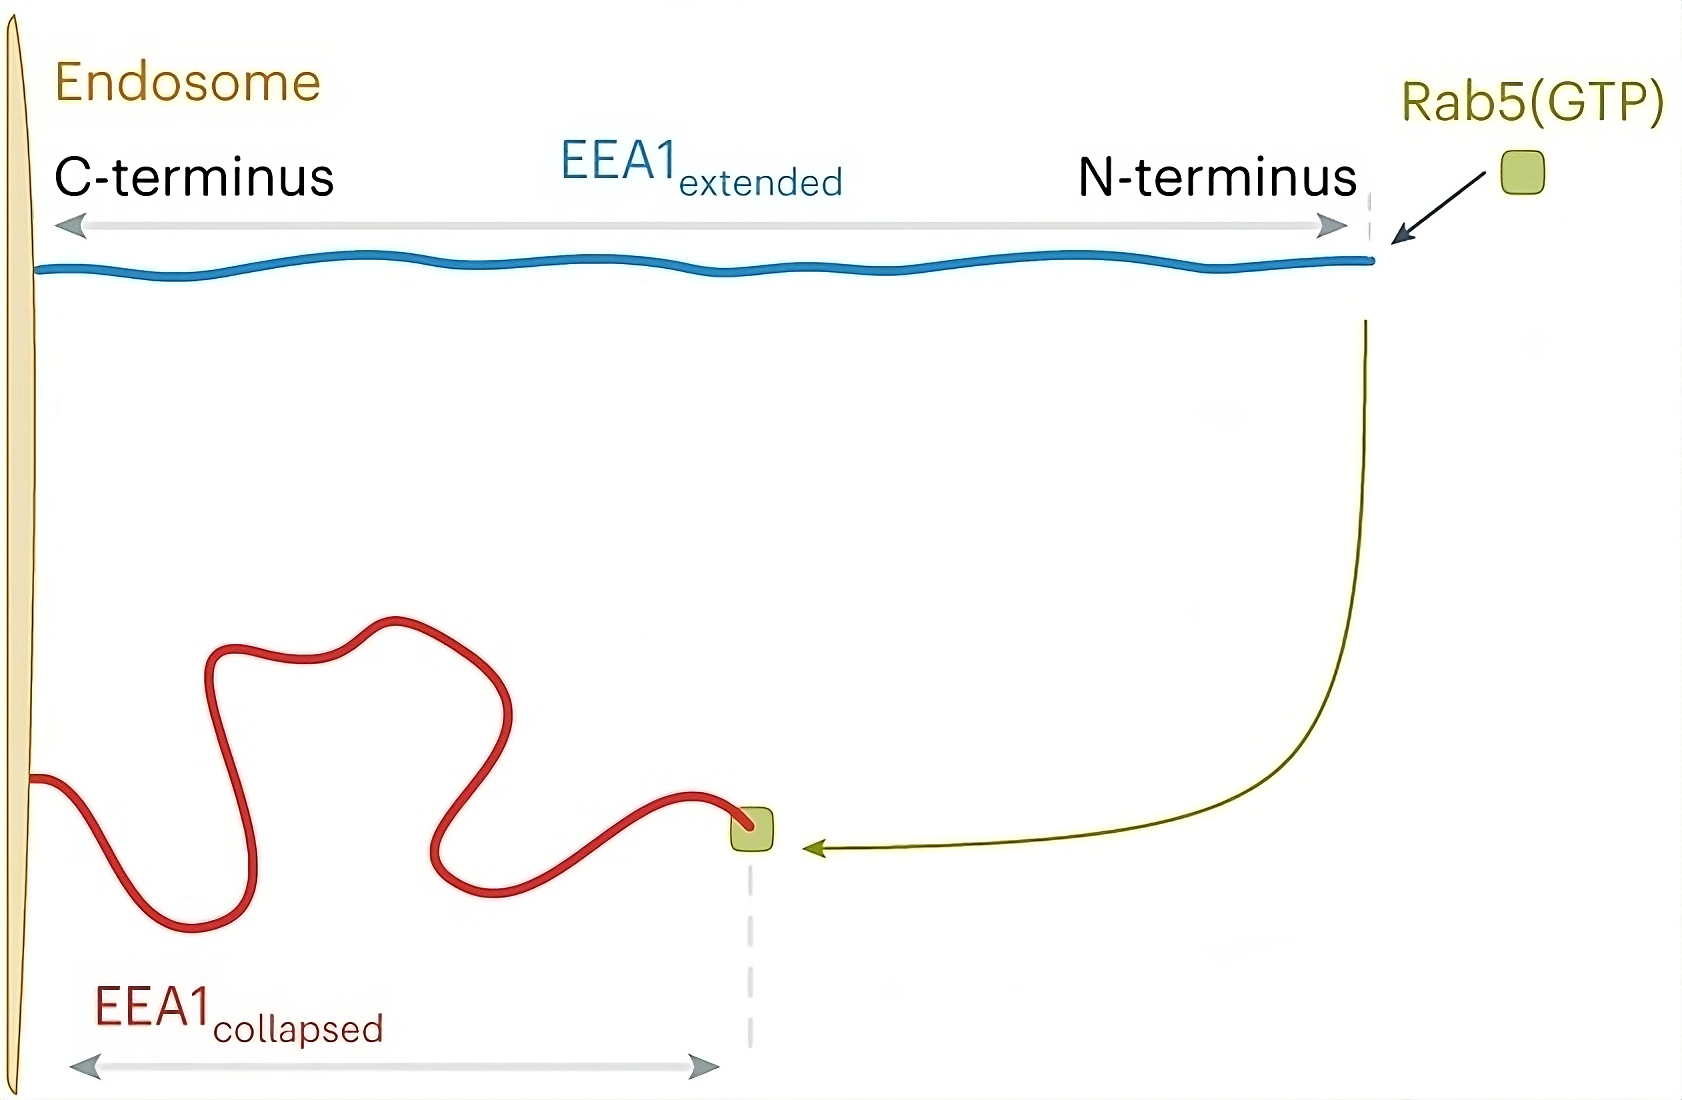
\includegraphics[height=6.9cm]{./Singh_intro_a.png}
        \caption{
            Sketch of extended/collapsed states of EEA1 upon the binding of Rab5
            \cite{Singh:2022}
        }
    \end{figure}
\end{frame}

% Motivation - Quantities ---------------------------------------------------------------------------

\begin{frame}
    \frametitle{Definitions}
    \framesubtitle{MSD and scaling exponent}
    \begin{itemize}
        \item Mean squared displacement (MSD) of the chain end (MSDLM):
        $$\E{[\Delta\vec{r}_N(t)]^2} := \E{[\vec{r}_N(t)-\vec{r}_N(0)]^2}$$
        \item (Local) scaling exponent alpha of the MSD \cite{Singh:2022}
        $$\E{[\Delta\vec{r}_N(t)]^2} \propto t^{\alpha(t)}$$
    \end{itemize}
\end{frame}

% Motivation - paper ---------------------------------------------------------------------------

\begin{frame}
    \frametitle{Motivation - experimental study}
    \framesubtitle{MSD and local scaling exponent}
    \centering
    \begin{figure}[h]
        \centering
        \begin{subfigure}[b]{0.49\textwidth}
            \centering
            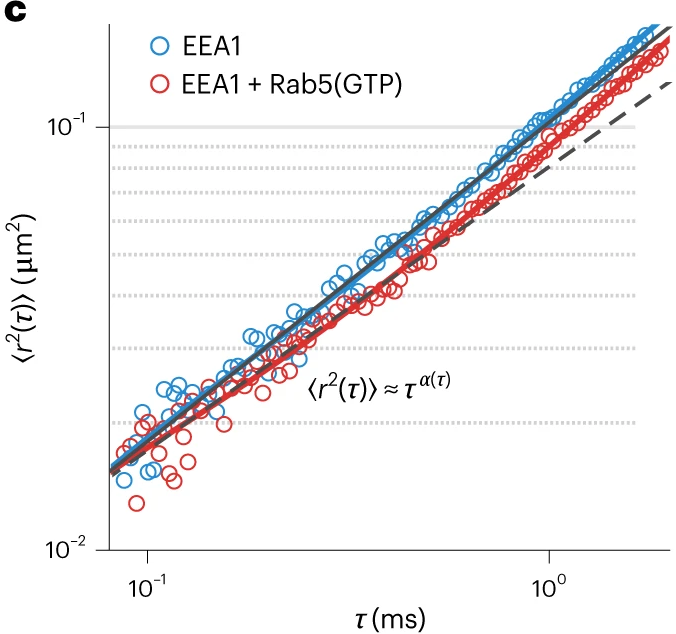
\includegraphics[width=\textwidth]{./Singh_intro_с.png}
        \end{subfigure}
        \begin{subfigure}[b]{0.49\textwidth}
            \centering
            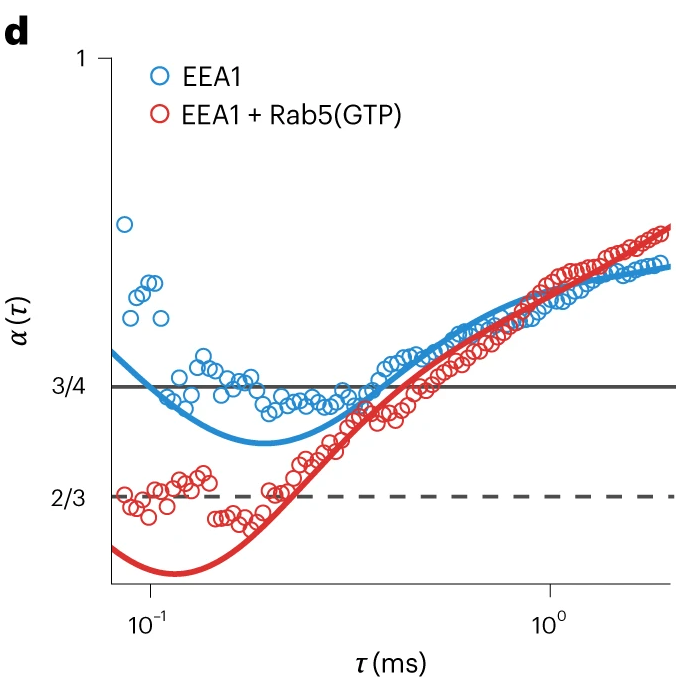
\includegraphics[width=\textwidth]{./Singh_intro_d.png}
        \end{subfigure}
        \caption{
            \textbf{c)} Mean square displacement (MSD) and \textbf{d)}
            local scaling exponent $\alpha$ of the MSD \cite{Singh:2022}
        }
    \end{figure}

\end{frame}

% Motivation - summary ---------------------------------------------------------------------------

\begin{frame}
    \frametitle{Motivation - summary}
    \begin{itemize}
        \item Change of stiffness is shown indirectly by fitting the 
        analytical expression to the experimentally observed data before/after
        the binding $\Rightarrow$ might be other impact factors (complex system)
        \item Free chains are measured, however by the membrane tethering the EEA1 
        chain is anchored to the endosome
        \item The dynamics of anchored semiflexible chains is not yet well studied 
    \end{itemize} 
\end{frame}

% Goals ---------------------------------------------------------------------------

\begin{frame}
    \frametitle{Introduction - Goals}

    Using the molecular dynamics:
    \vspace{0.5cm}
    \begin{itemize}
        \item Study dynamical properties of the anchored
        semiflexible chains by varying stiffness and friction of the chain end
        \item Change in mechanical properties (chain stiffness, friction coefficient of the chain end)
        "$\Rightarrow$" change in scaling behavior of the MSD as in \cite{Singh:2022}? 
    \end{itemize}

\end{frame}

% Limitations ---------------------------------------------------------------------------

\begin{frame}
    \frametitle{Introduction - Limitations}

    \begin{itemize}
        \item No hydrodynamic interactions
        \item Ideal chains
    \end{itemize}

\end{frame}

% Methods ---------------------------------------------------------------------------

\begin{frame}
    \frametitle{Introduction - Methods}
    \framesubtitle{Molecular dynamics}
    \centering
    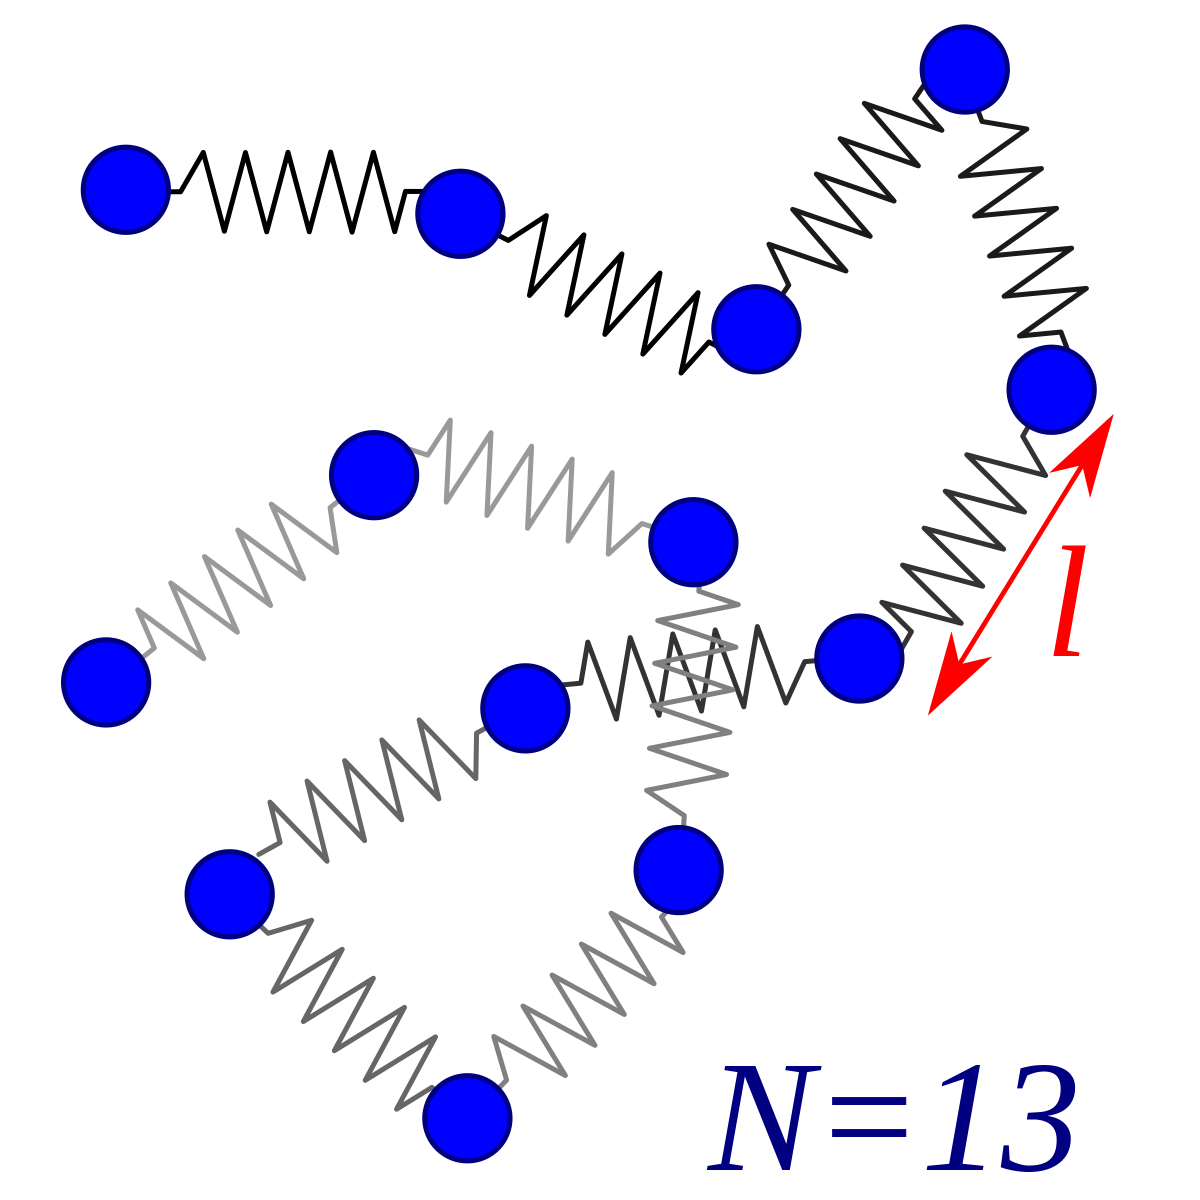
\includegraphics[width=0.3\textwidth]{./bead_spring_model.png}
    \begin{itemize}
        \item Model the polymer chain as series of interconnected beads
        \item Bond potential to model the interaction of bonded beads
        \item In case of anchored chains fix the position of first 2 beads
        \item Angle potential to model the stiffness of the chain
        \item Random force + damping to model the solvent
        \item Time-integrate the equations of motion
    \end{itemize}
    
\end{frame}

\section{Anchored chain dynamics}


% Fully flexible anchored ---------------------------------------------------------------------------


\subsection{Comparison to free chain}

\begin{frame}
    \frametitle{Anchored fully flexible chains}
    \framesubtitle{Definitions, notations, equations}
    \begin{itemize}
        \item MSD of End-to-End distance (MSD of ETE): 
        $$ \E{[\Delta \vec{R}(t)]^2} := \E{[\vec{R}(t)-\vec{R}(0)]^2} $$
        \item Contour length: $L$, Friction coefficient of the bead: $\zeta$,
        Bond length: $l_b$, Number of beads: $N$
        \item Rouse model predictions for MSD of ETE of free fully flexible chain:
        $$\E{[\Delta \vec{R}(t)]^2} = f(t; \tau_R, \E{R})$$
        with characteristic time time scale, Rouse time: $$\tau_R(N,l_b,\zeta)$$
    \end{itemize}
    
\end{frame}


\begin{frame}
    \frametitle{Anchored fully flexible chains}
    \framesubtitle{MSD of ETE: $\mean{[\Delta R(t)]^2}$ - free vs anchored chains}

    \begin{figure}[h]
        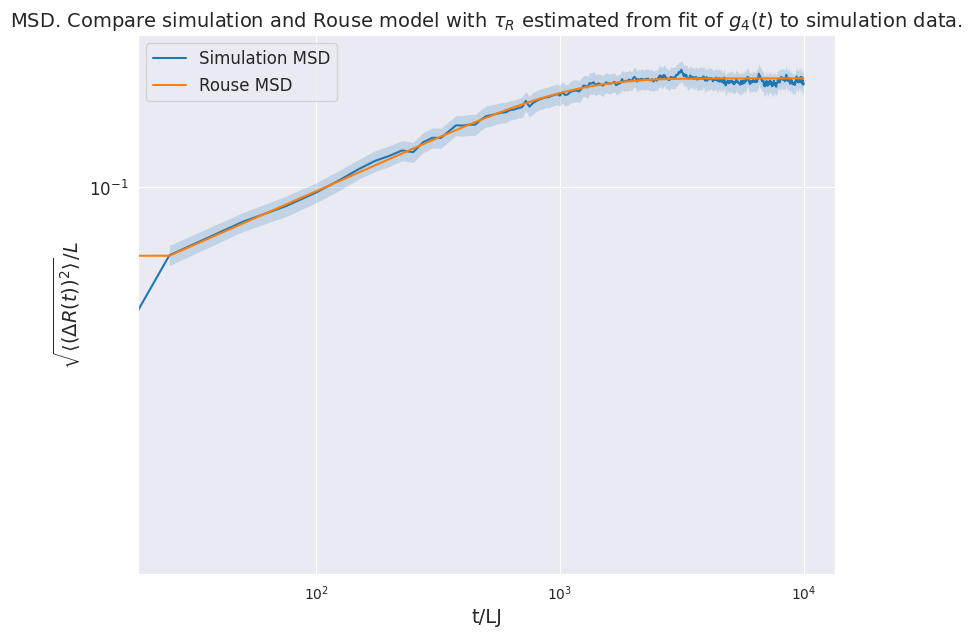
\includegraphics[trim={0.1cm 0.1cm 0.1cm 1cm},clip,width=\textwidth]{./3-exp-free-param-log.png}
        \caption{
            MSD of ETE - compare simulation of free chains, anchored chains and Rouse model,
            $\frac{\tau_{R, \textrm{empirical,anchored}}}{\tau_{R, \textrm{analytical, free}}} \approx 4$
        }
        \label{fig:full-flex-chain-free-log}
    \end{figure}
\end{frame}

\subsection{Impact of chain stiffness}

% Semiflexible anchored - Equations -------------------------------------------------------------------

\begin{frame}
    \frametitle{Anchored semiflexible chains - impact of stiffness}
    \framesubtitle{Definitions, equations, notations}
    \begin{itemize}
        \item Persistence length: $l_p$
        \item Kuhn length $l_K=2l_p=g(\text{angle potential paramater}, l_b)$
    \end{itemize}
\end{frame}

% Semiflexible anchored - MSD ---------------------------------------------------------------------------

\begin{frame}
    \frametitle{Anchored semiflexible chains - impact of stiffness}
    \framesubtitle{MSD of ETE: $\mean{[\Delta \vec{R}(t)]^2}$ for different $l_K$ values}

    \begin{figure}
        \centering
        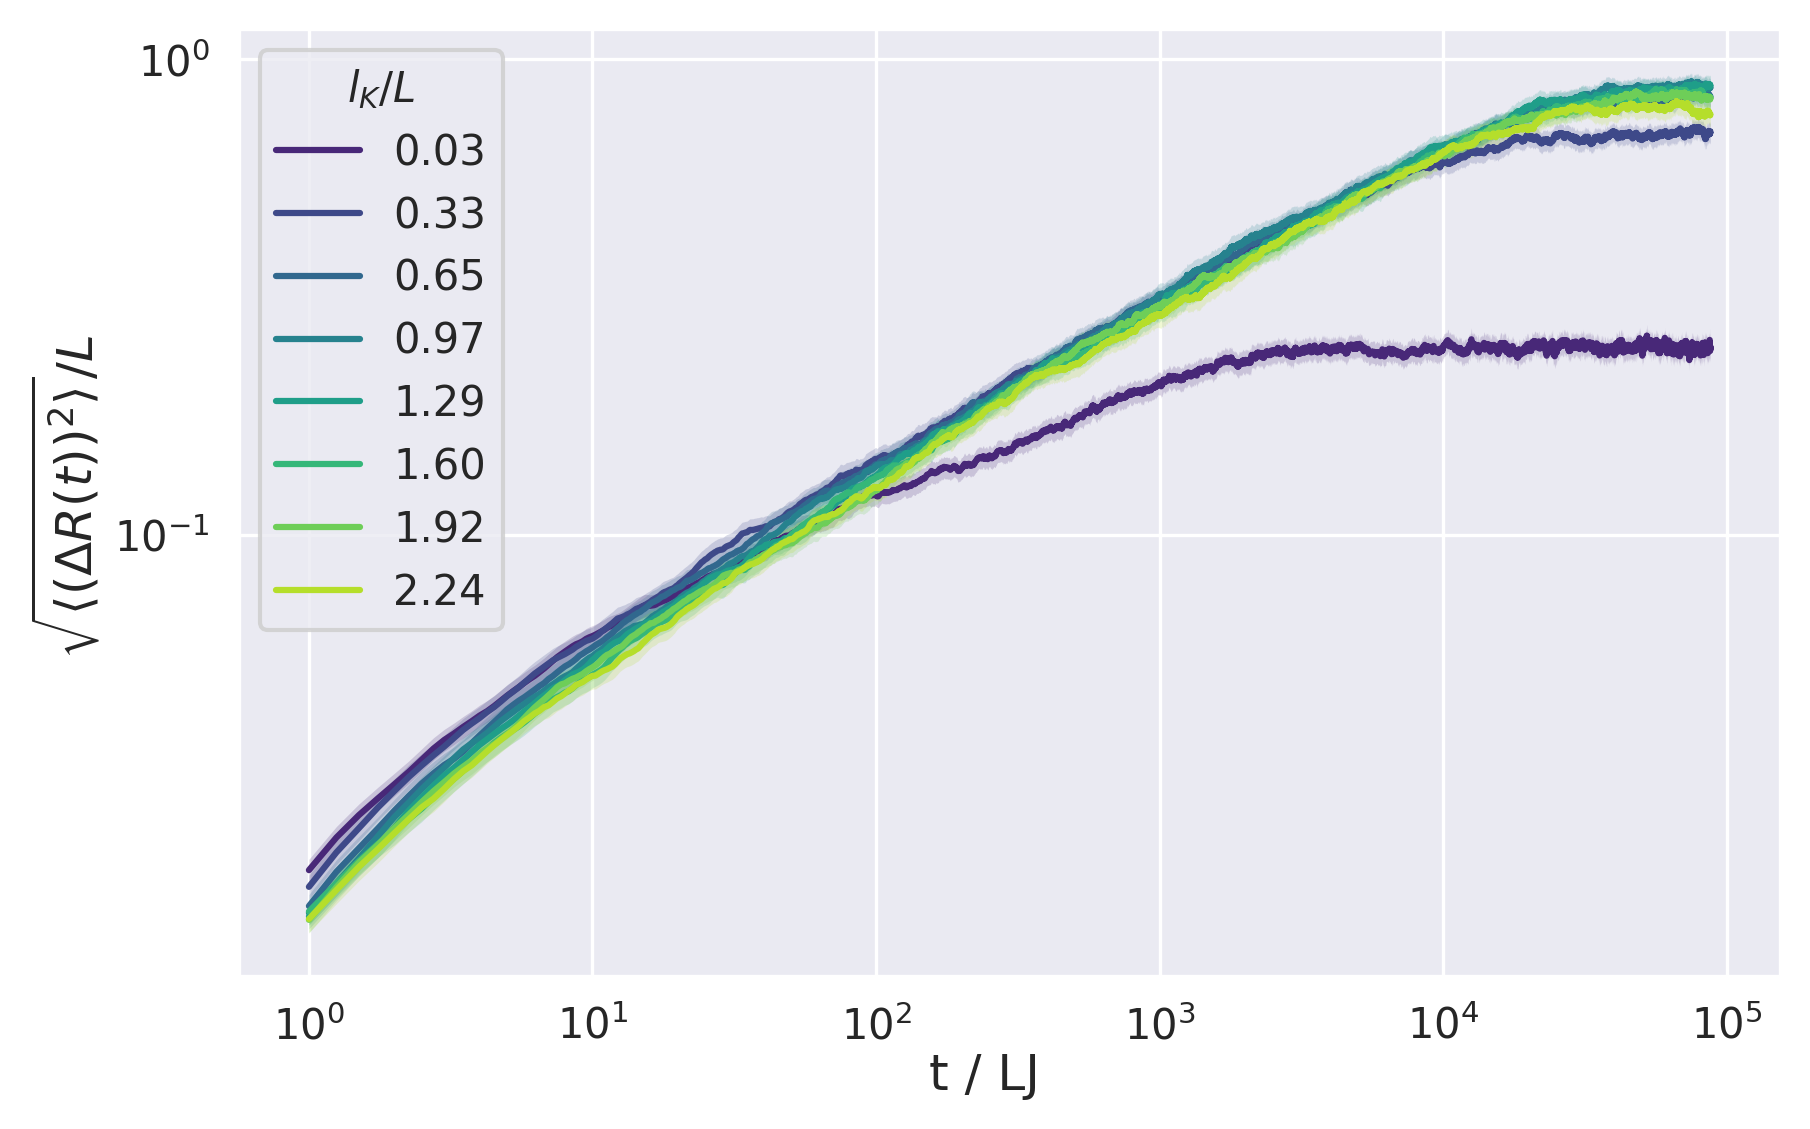
\includegraphics[width=\columnwidth,trim={0cm 0cm 0cm 0.0cm},clip]{4-exp-delta_R-bare-log.png}
        \caption{Empirical MSD of ETE of anchored chains with different Kuhn length values.}
        \label{fig:msd_anchored_l_K}
    \end{figure}
\end{frame}

% Semiflexible anchored - Equations -------------------------------------------------------------------

\begin{frame}
    \frametitle{Anchored semiflexible chains - impact of stiffness}
    \framesubtitle{Attemp analytical description, Quantify difference, "Adjusted Rouse model" definition}
    For anchored semiflexible chains assume:
    $$ \mean{[\Delta \vec{R}(t)]^2} = h(t; \tau_{rot}, a, \E{R}) = a \mean{R} [1 - \exp(-\frac{t}{\tau_{rot}})]$$
    with $\tau_{rot}$ and $a$ - free parameters.
    \begin{itemize}
        \item Based on Rouse model predictions for free semiflexible chains, 
        long time limit
        \item $\tau_{rot}$ characteristic time scale, may have different meaning
        then in case of free semiflexible chains.
    \end{itemize}
\end{frame}

% Semiflexible anchored - MSD vs Adjusted Rouse ---------------------------------------------------------------------------

\begin{frame}
    \frametitle{Anchored semiflexible chains - impact of stiffness}
    \framesubtitle{MSD $\mean{[\Delta \vec{R}(t)]^2}$ vs Adjusted Rouse with $\tau_R$, $a$ as free parameters}
    \begin{figure}[h]
        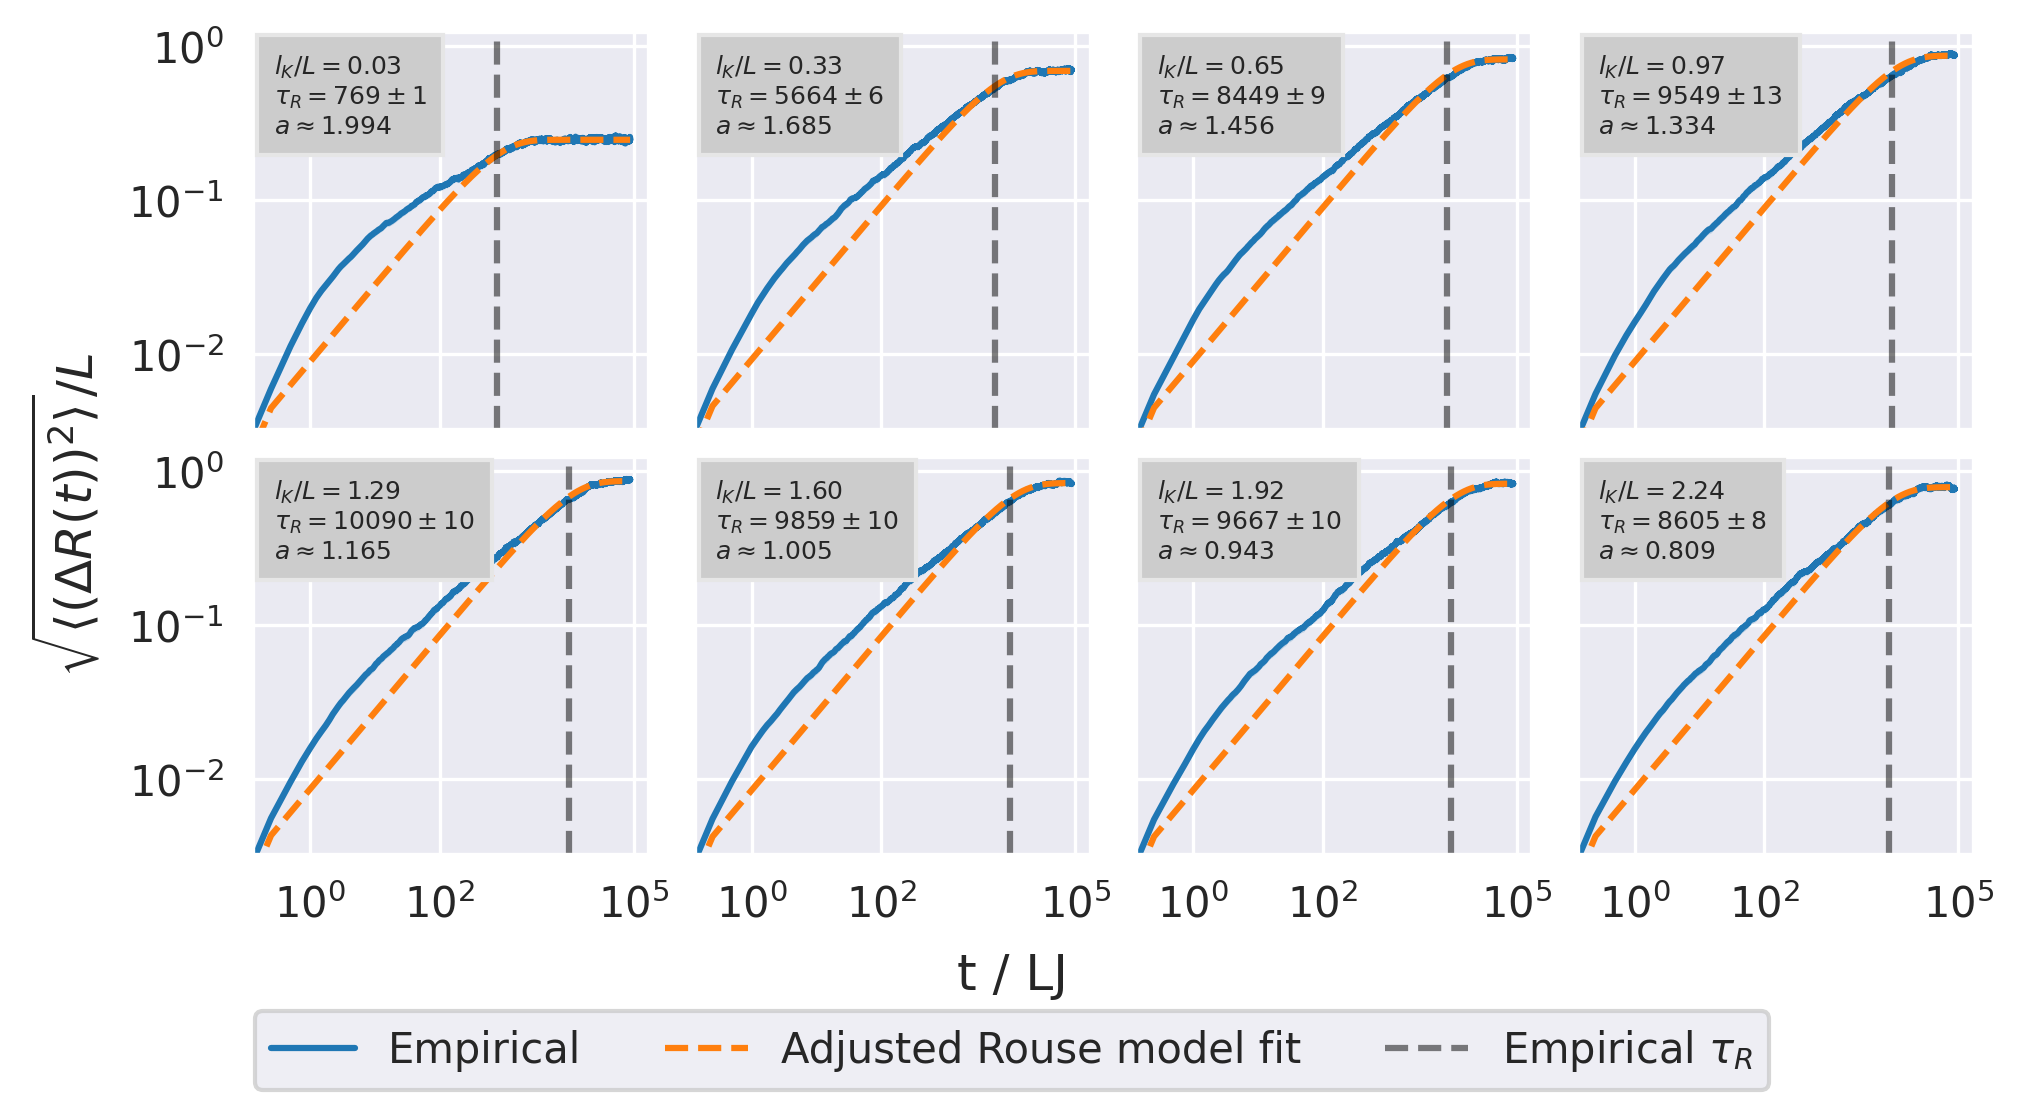
\includegraphics[width=11cm]{4-exp-delta_R-rouse_fit-tau-a_log.png}
        \caption{MSD of ETE of anchored semiflexible chains compared to 
        "Adjusted Rouse model"}
    \end{figure}
\end{frame}

% Semiflexible anchored - alpha assumtion ---------------------------------------------------------------------------

\begin{frame}
    \frametitle{Anchored semiflexible chains - impact of stiffness}
    \framesubtitle{Define local scaling exponent}
    For the anchored chains is assumed, that:
    $$\mean{[\Delta \vec{R}(t)]^2} \propto t^{\alpha(t)}$$
    which defines the (local) scaling exponent $\alpha$
    for the case of anchored chains.
    

\end{frame}

% Semiflexible anchored - alpha ---------------------------------------------------------------------------

\begin{frame}
    \frametitle{Anchored semiflexible chains - impact of stiffness}
    \framesubtitle{Scaling behavior}
    \begin{figure}[h]
        \begin{center}
          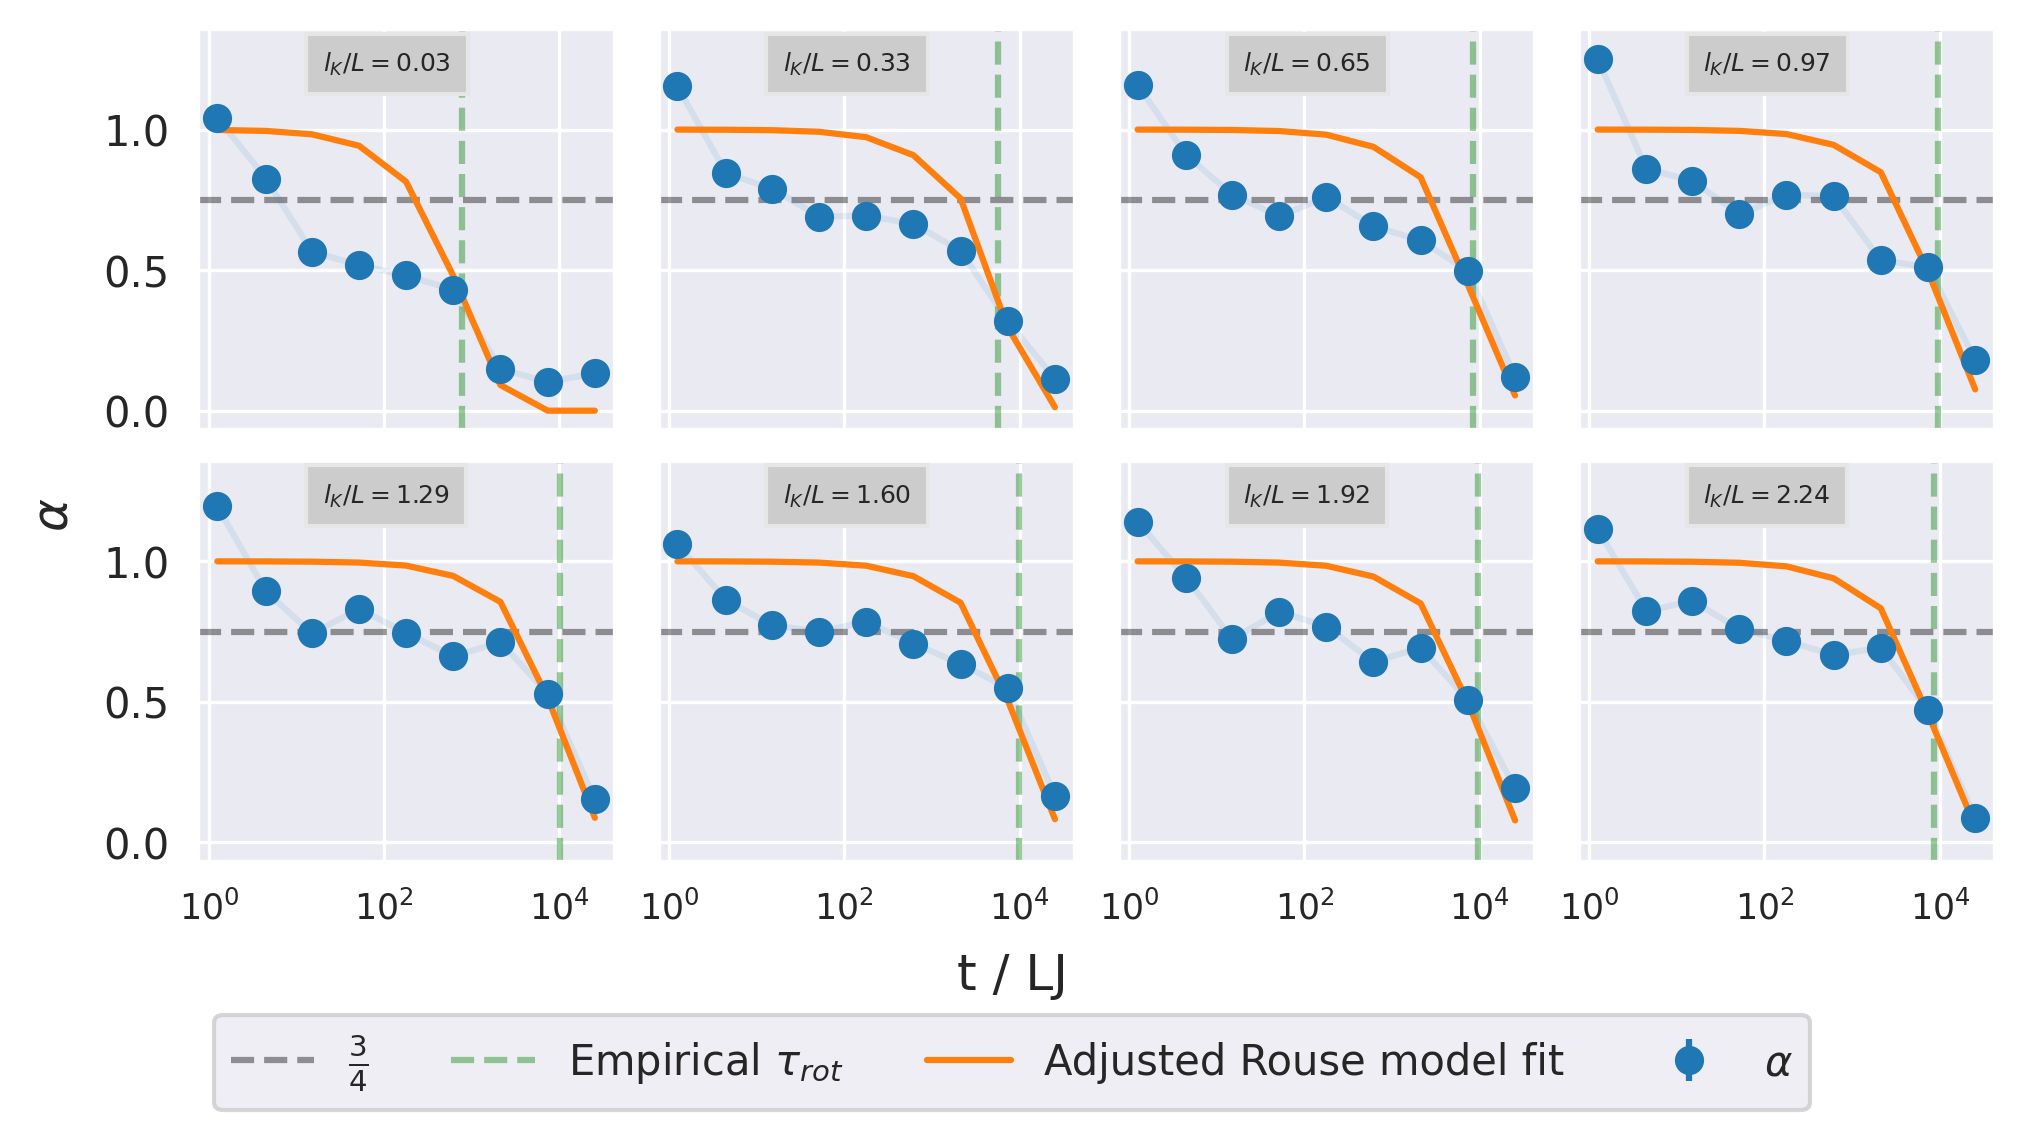
\includegraphics[width=\columnwidth,trim={0cm 0cm 0cm 0.0cm},clip]{4-exp-delta_R-rouse_fit-tau-a_alpha.png}
          \caption{\label{fig:alpha_anchored_l_K}
          Scaling exponent $\alpha$ of the MSD of ETE of anchored semiflexible chain (blue points) and 
          scaling exponent $\alpha$ of the Adjusted Rouse model prediction for semi-flexible chains 
          (orange line).
          }
        \end{center}
    \end{figure}
\end{frame}

\subsection{Impact of the friction coefficient of the chain end}

% Semiflexible anchored impact of zeta_e - intro ----------------------------------------

\begin{frame}
    \frametitle{Anchored semiflexible chains - impact of $\zeta_e$}
    \framesubtitle{Notations}
    \begin{itemize}
        \item index "e" for variables referring end-monomer of the chain: $m_e$, $\zeta_e$ 
    \end{itemize}
\end{frame}

% Semiflexible anchored impact of zeta_e - compare params ----------------------------------------

\begin{frame}
    \frametitle{Anchored semiflexible chains - impact of $\zeta_e$}
    \framesubtitle{MSD, compare parameters}
    \begin{figure}[h]
        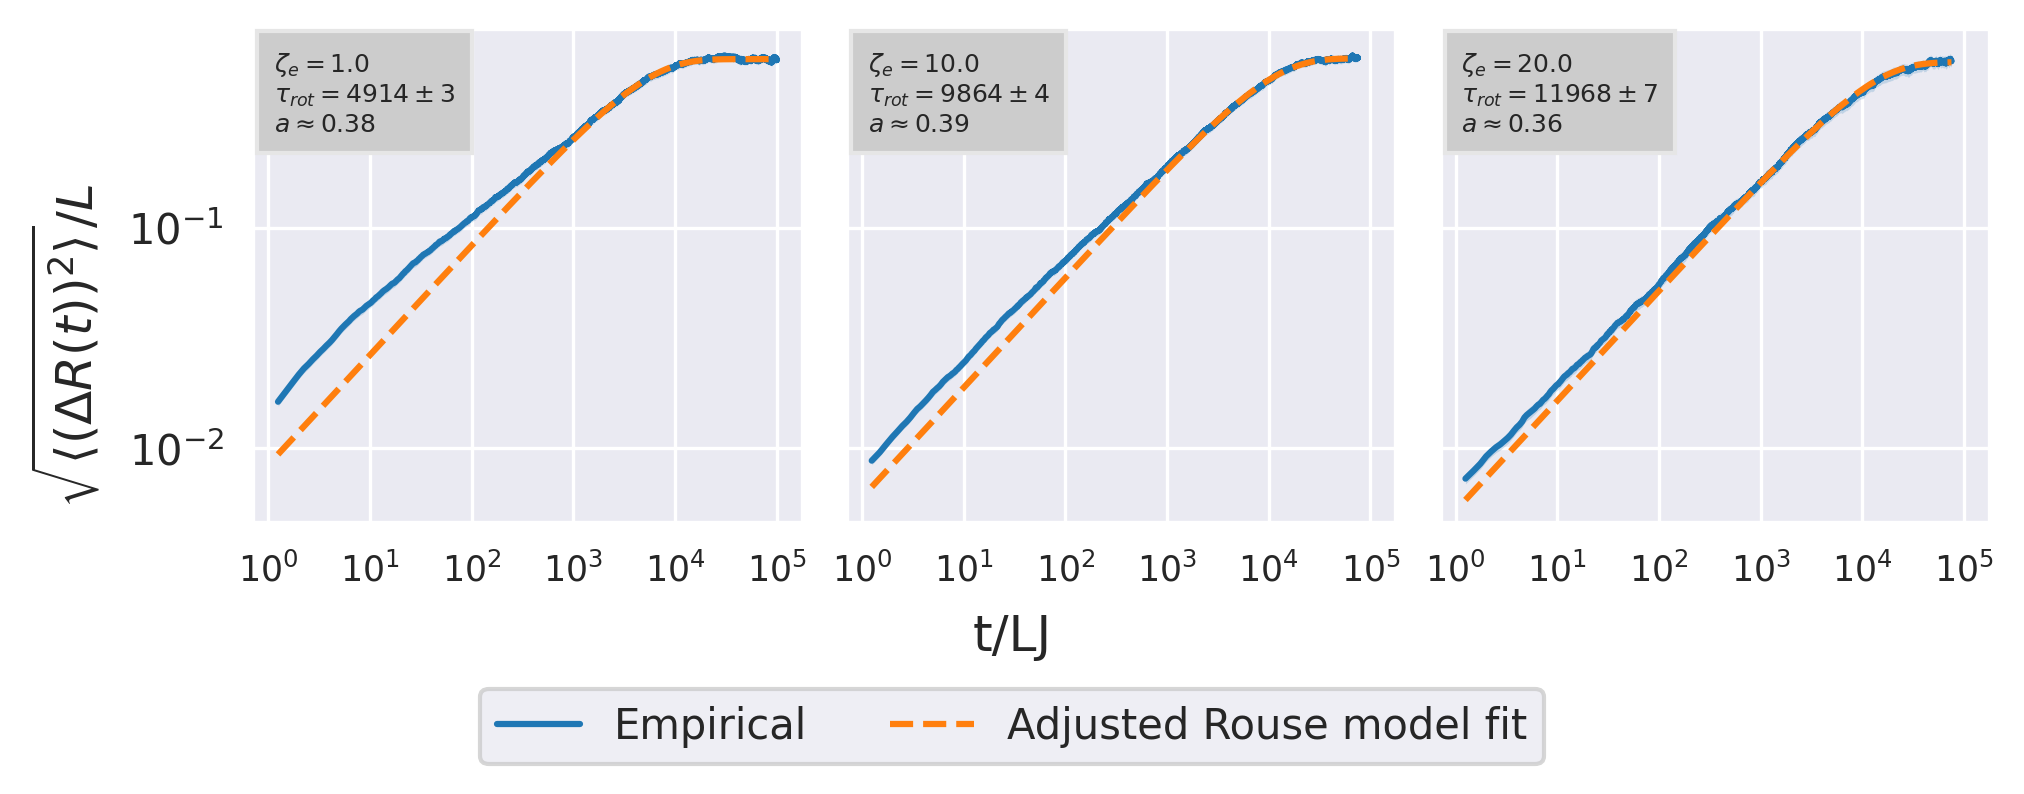
\includegraphics[width=\textwidth]{14+15+16-exp-msd-log-arm_fit-log.png}
        \caption{Empirical MSD of ETE of anchored chains with different values of
        the friction coefficient of the chain end $\zeta_e$ and a corresponding fit
        of the Adjusted Rouse model.
        }
    \end{figure}
\end{frame}

% Semiflexible anchored impact of zeta_e - alpha ----------------------------------------

\begin{frame}
    \frametitle{Anchored semiflexible chains - impact of $\zeta_e$}
    \framesubtitle{Scaling behavior}
    \begin{figure}[h]
        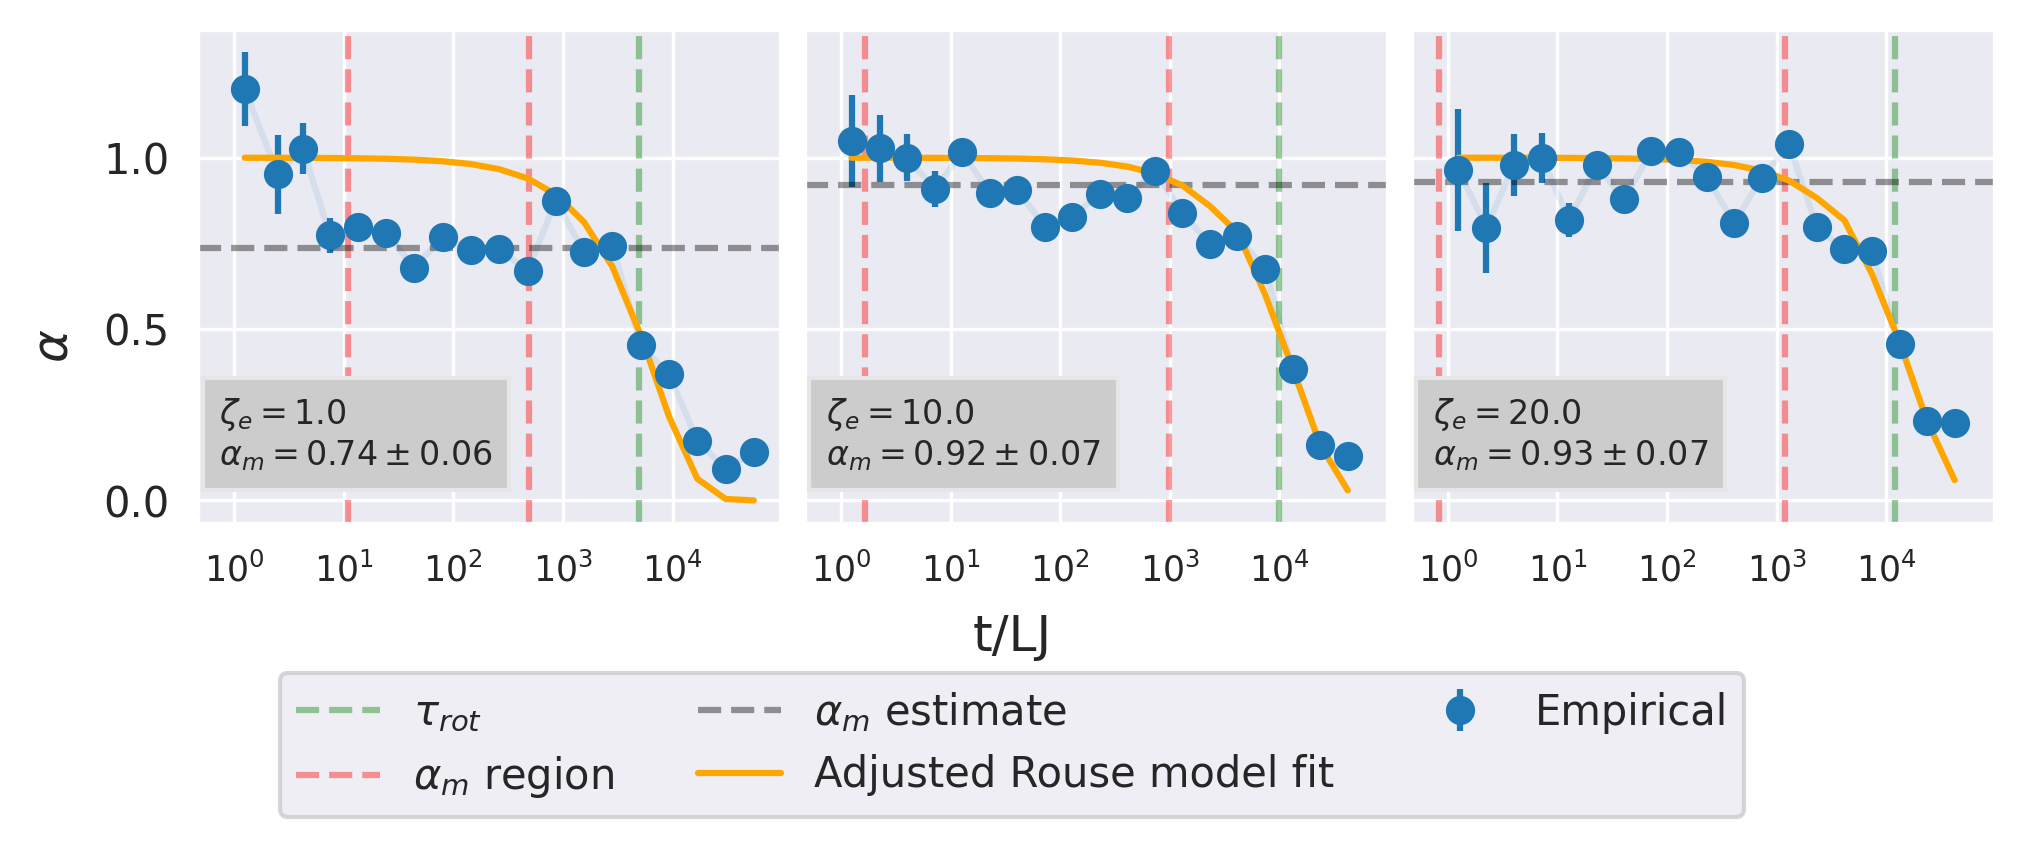
\includegraphics[width=\textwidth]{14+15+16-exp-alpha.png}
        \caption{Scaling exponent $\alpha$ of MSD of ETE 
        of anchored chains with different values of
        friction coefficient of the chain end $\zeta_e$ (blue dots).
        Estimated scaling exponent for the time interval
        $t \ll \tau_{rot}$: $\alpha_m$ (grey dashed line); Red dashed lines
        correspond to $\alpha_m$ scaling region which is estimated as:
        $[10 \frac{m_e}{\zeta_e}, \frac{\tau_{rot}}{10}]$
        }
    \end{figure}
\end{frame}


\section{Free chain dynamics}

% Free, smaller end - MSD ----------------------------------------

\begin{frame}
    \frametitle{Free chains}
    \framesubtitle{MSDLM, smaller chain end}
    \begin{figure}[h]
        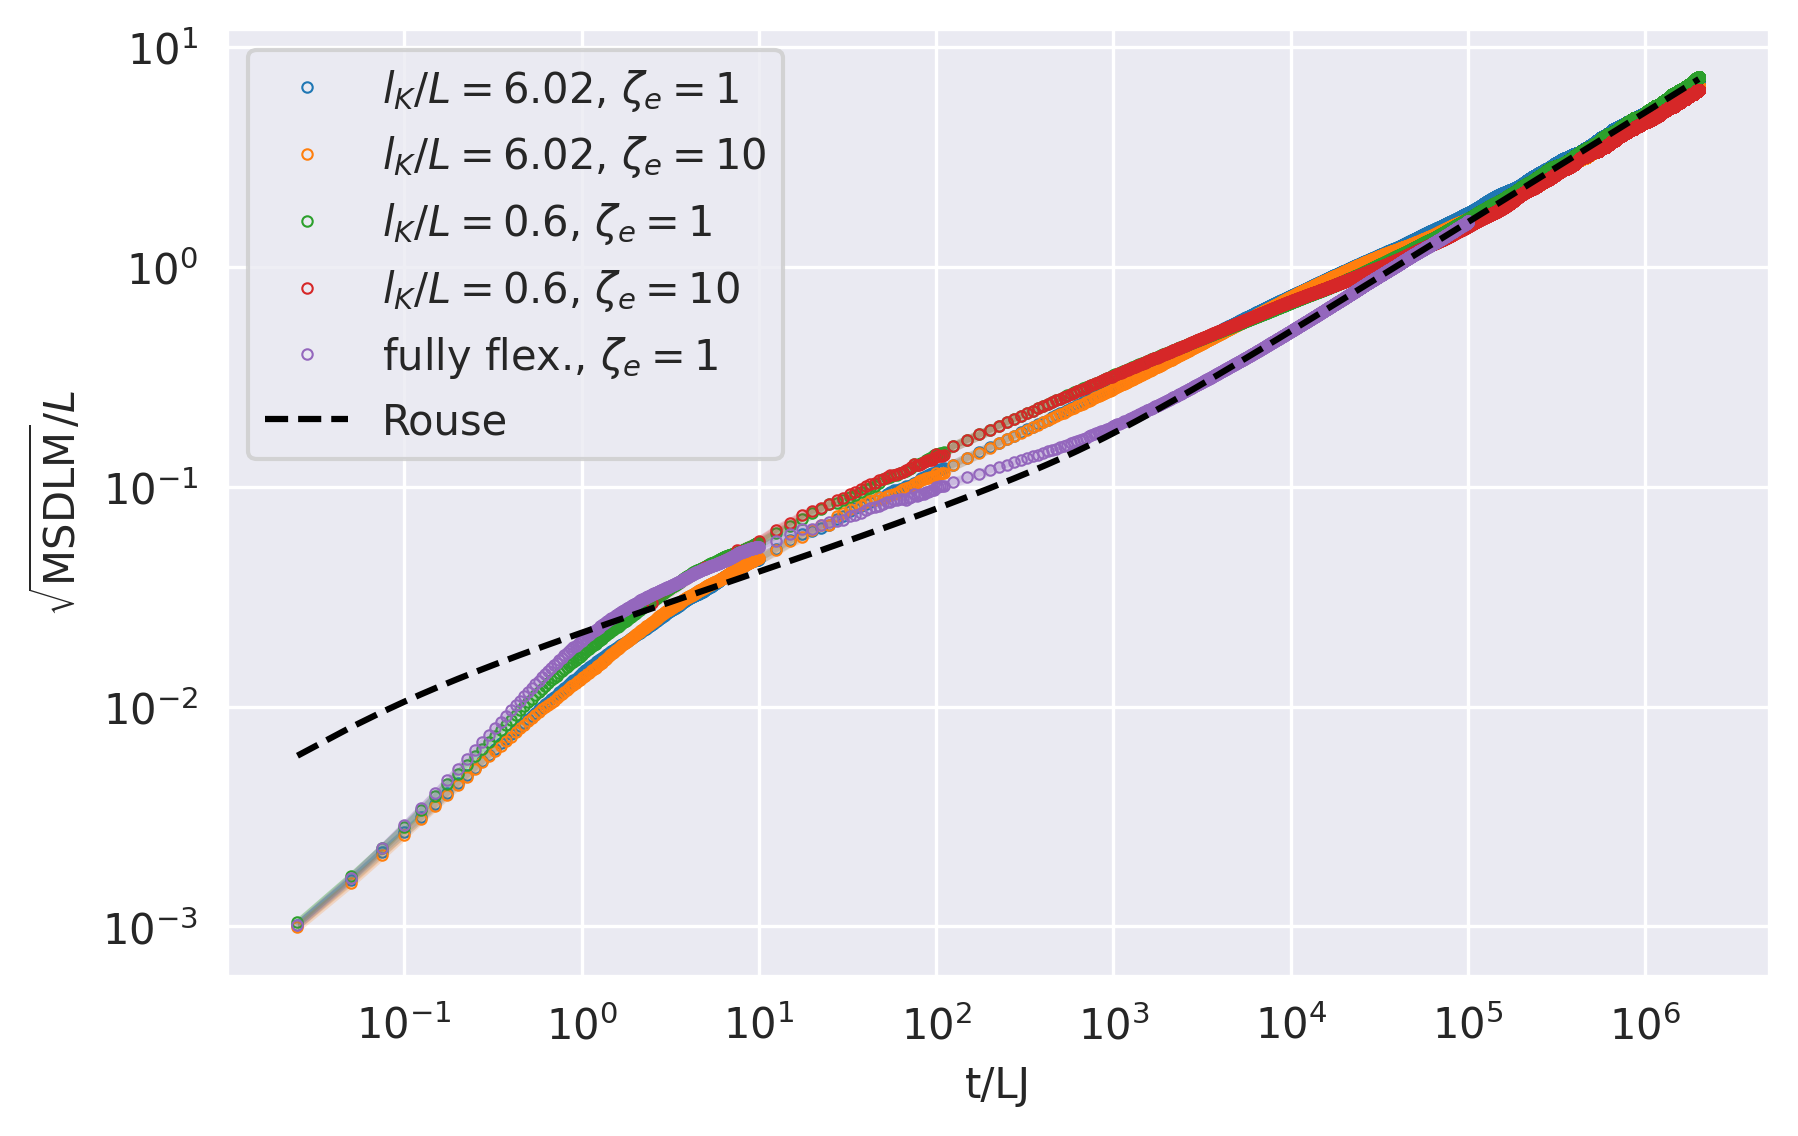
\includegraphics[width=0.9\textwidth]{17+18+19+20-exp-msd-fm-log.png}
        \caption{
            Empirical MSD of chain end (MSDLM) of free chains
            with different stiffness and end-bead friction values and
            Rouse model prediction for fully flexible chains.
        }
    \end{figure}
\end{frame}

% Free, smaller end - alpha ----------------------------------------

\begin{frame}
    \frametitle{Free chains}
    \framesubtitle{Scaling behavior, smaller chain end}
    \begin{figure}
        \centering
        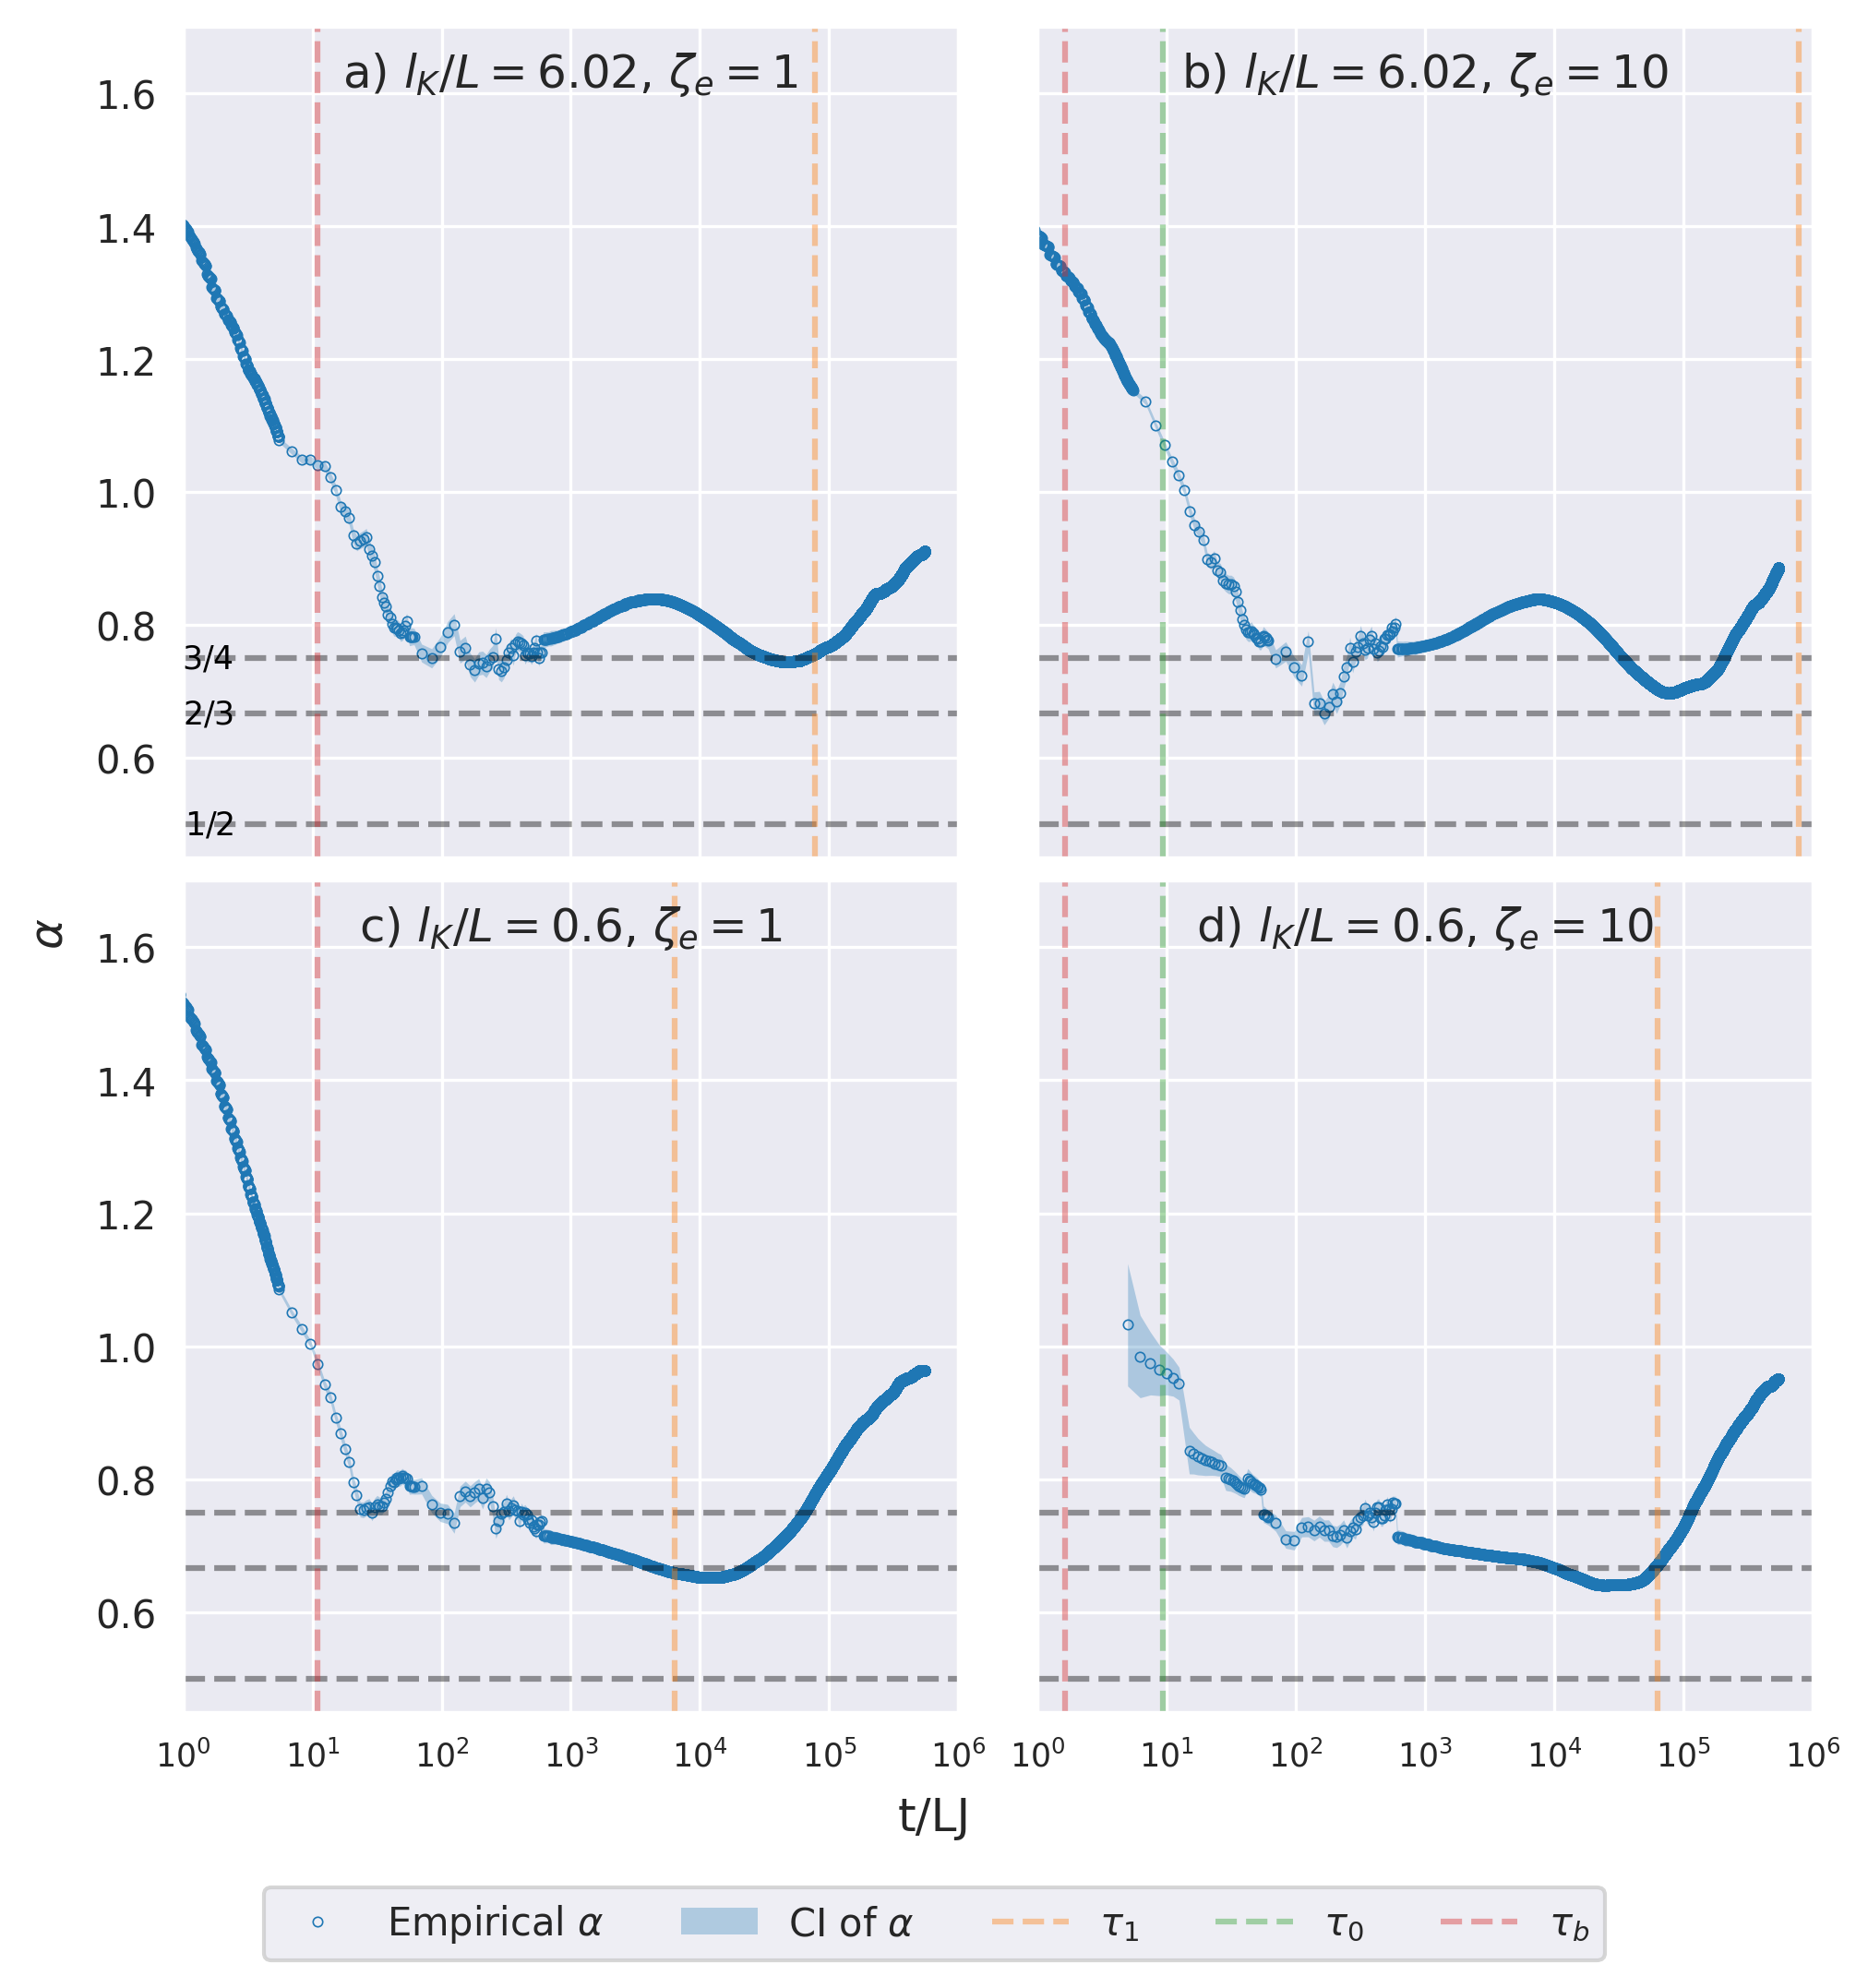
\includegraphics[width=0.6\textwidth]{17+18+19+20-exp-alpha-fm.png}
        \caption{Scaling exponent $\alpha$ of MSD of chain end (MSDLM) 
        of free chains with different stiffness and end-bead friction values
        }
        \label{fig:alpha_fm_free}
    \end{figure}
\end{frame}

% Free, smaller end - change of alpha -------------------------------------------

\begin{frame}
    \frametitle{Free chains}
    \framesubtitle{Scaling behavior, smaller chain end}
    \begin{figure}
        \centering
        \begin{subfigure}{0.58\textwidth}
            \centering
            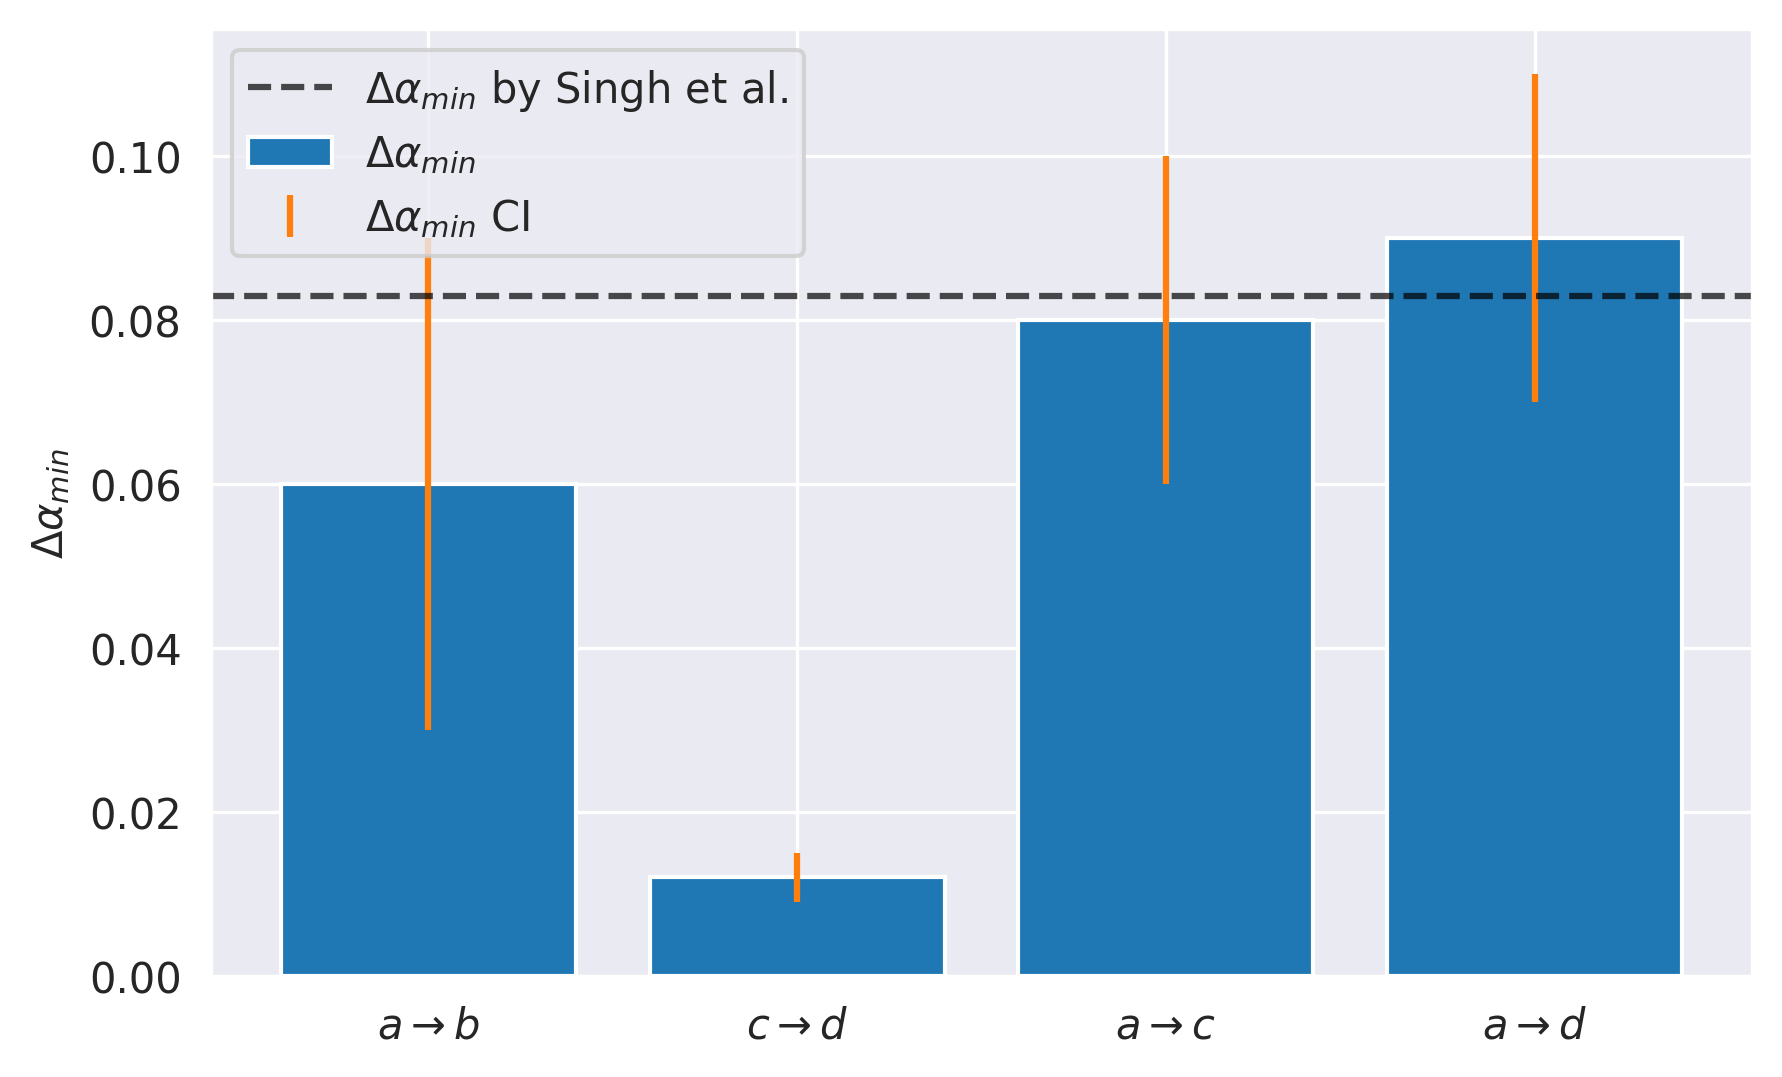
\includegraphics[width=\textwidth]{17+18+19+20-exp-delta_alpha_min_fm.png}
        \end{subfigure}
        \begin{subfigure}{0.4\textwidth}
            \centering
            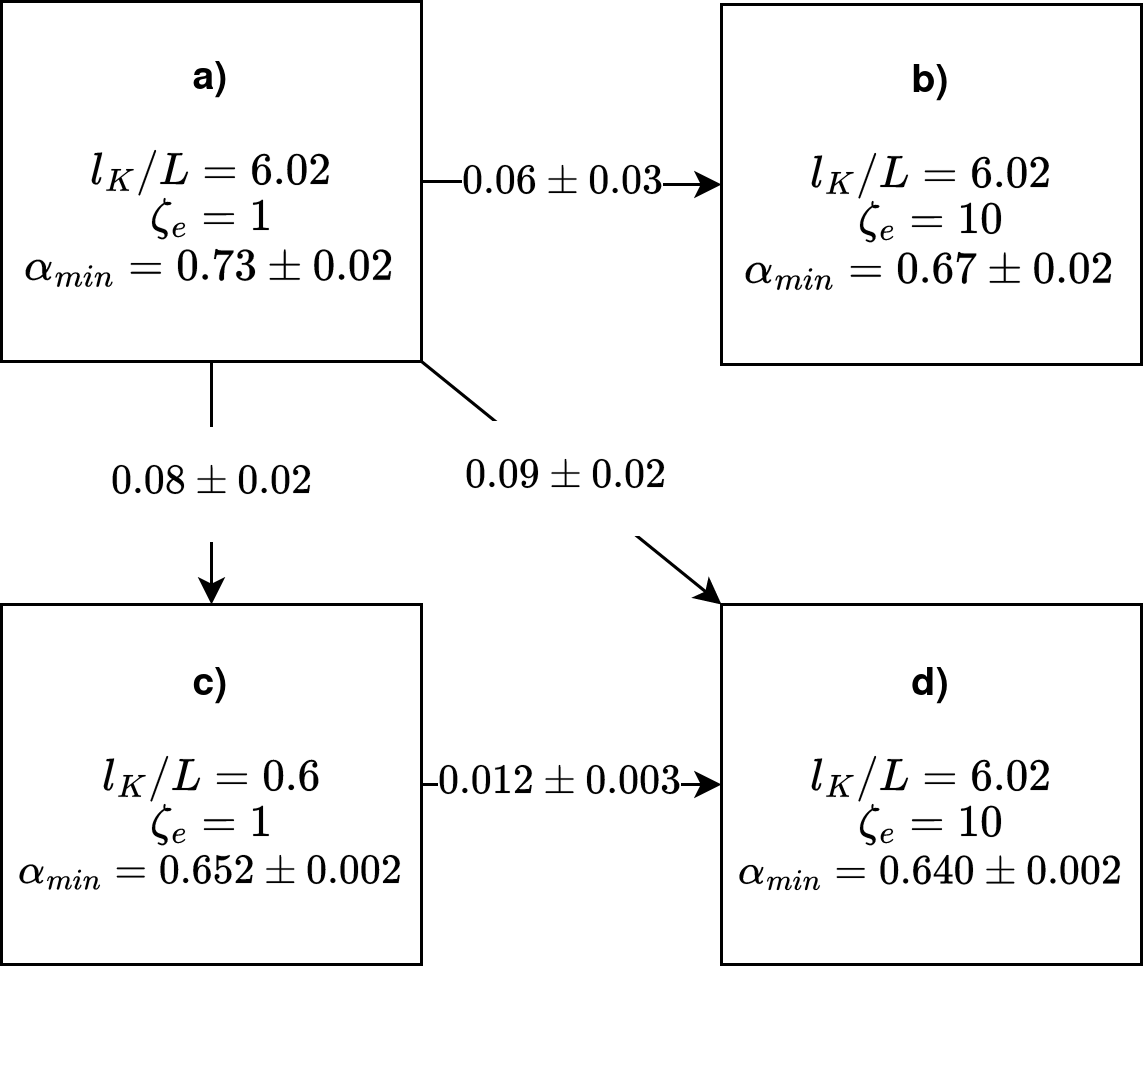
\includegraphics[width=\textwidth]{cases_diag.png}
        \end{subfigure}
        \caption{
            Change of scaling exponent $\alpha$ of MSD of chain end (MSDLM)
            of free chains by the change of $l_K$ and $\zeta_e$.
        }
    \end{figure}
\end{frame}

\section{Summary}

% Summary - what is done -------------------------------------------


\begin{frame}
    \frametitle{Summary - what is done}
    With help of molecular dynamics simulations:
    \begin{itemize}
        \item Measured and analyzed MSD of ETE of anchored chains for range of
        stiffness and friction coefficient of chain end values
        \item{Measured and analyzed MSD of chain end of free chains for several specific
        stiffness and friction coefficient of the chain end values}
    \end{itemize}
    under the assumption of ideal chains and absence of hydrodynamic interactions.
\end{frame}

% Summary - conslusions -------------------------------------------

\begin{frame}
    \frametitle{Summary - conclusions}
    \framesubtitle{Anchored chains - effects of anchoring}
    \begin{itemize}
        \item Anchoring of fully flexible chain $\Rightarrow$ ~4x increase of characteristic
        time: $\tau_R$ (Rouse relaxation time)
    \end{itemize}
\end{frame}

\begin{frame}
    \frametitle{Summary - conclusions}
    \framesubtitle{Anchored chains - impact of stiffness}
    \begin{itemize}
        \item Exponential decrease of MSD of ETE of anchored semiflexible chains
        after estimated characteristic time $\tau_{rot}$, which increases
        with growing stiffness
        \item The values of $\alpha(t)$ in the region of subdiffusive motion
        qualitatively correspond to ones predicted for the free chain,
        moving from $1/2$ to $3/4$.
    \end{itemize}
\end{frame}

\begin{frame}
    \frametitle{Summary - conclusions}
    \framesubtitle{Anchored chains - impact of friction coefficient of chain end $\zeta_e$}
    \begin{itemize}
        \item Increase of an estimated characteristic time $\tau_{rot}$ 
        with increase of $\zeta_e$
        \item By an increase of $\zeta_e$ from $1$ to $10$ the value of $\alpha(t)$ in the region
        of subdiffusive motion increases
        \item By the further increase $\zeta_e$ (from $10$ to $20$) the value of $\alpha(t)$ in the region
        of subdiffusive motion remains roughly the same
    \end{itemize}
\end{frame}

\begin{frame}
    \frametitle{Summary - conclusions}
    \framesubtitle{Free chains}
    \begin{itemize}
        \item Both, stiffness decrease and increase of $\zeta_e$ can cause a decrease
        of the minimum of scaling exponent $\alpha(t)$ of MSD
        \item There are hints, that increase of $\zeta_e$ alone is not enough for
        large enough (0.08, as observed by Singh et al.) decrease of the minimum of scaling exponent $\alpha(t)$ 
    \end{itemize}
\end{frame}

% Summary - outlook -------------------------------------------

\begin{frame}
    \frametitle{Summary - outlook}
    \begin{itemize}
        \item Consider hydrodynamic and excluded volume interactions
        \item Explore value of $\zeta_e$ matching Rab5
        \item Grid of $\l_p$ and $\zeta_e$ values to obtain curves
        of characteristic times and minimas of scaling exponent in dependence of
        $l_p$ and $\zeta_e$
        \item Increase number of beads to better match $l_b \ll L$ and
        length of EEA1 chain
    \end{itemize}
\end{frame}

\section{References}

% references -------------------------------------------

\setbeamertemplate{bibliography item}{\insertbiblabel}
\begin{frame}
    \frametitle{References}
    \bibliographystyle{apalike}
    \bibliography{sources}
\end{frame}

% appendix -----------------------------------------------------------------

\section{Appendix}

\begin{frame}
    \frametitle{Common simulation settings and values}

    \begin{itemize}
        \item Only bonded beads interract (ideal chain)
        \item Chain parameters: 64 monomers, monomer mass $m=1$
        \item Ensemble size $ \ge $ 500 chains
        \item Environment parameters: $\zeta=1$
        \item Time step 0.0025 LJ
    \end{itemize}

\end{frame}

\end{document}